\begin{frame}
	\frametitle{LDA - dimension reduction}
Steps:
\begin{enumerate}
	\item within-class scatter matrix for each class
	%
	\begin{equation}
	\Sigma_i = \frac{1}{N_{i}-1} \sum\limits_{\pmb x \in D_i}^n (\pmb x - \pmb \mu_i)\;(\pmb x - \pmb \mu_i)^T
	\end{equation} 
	then sum them to obtain
	%
	\begin{equation}
	\Sigma_W = \sum\limits_{i =1}^{n} (N_i - 1) \Sigma_i 
	\end{equation}
	
	\item between-class scatter matrix
	 \begin{equation}
	\Sigma_B = \sum\limits_{i =1}^n \dfrac{N_i}{N} (\pmb \mu_i - \pmb \mu) (\pmb \mu_i - \pmb \mu)^T
	\end{equation}
	
	\item find eigenvectors and eigenvalues of $\Sigma^{-1} \Sigma_b$
	\item using the eigenvectors we transform our data onto a new subspace
\end{enumerate}
\end{frame}

\begin{frame}
\frametitle{PCA vs LDA}
\begin{center}
	\centering
	\subfloat{{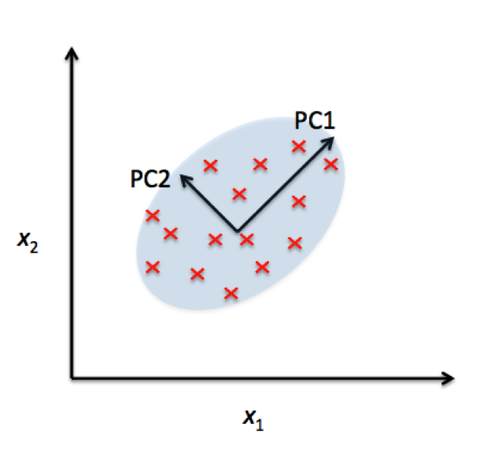
\includegraphics[width=0.4\columnwidth]{pca} }}
	\subfloat{{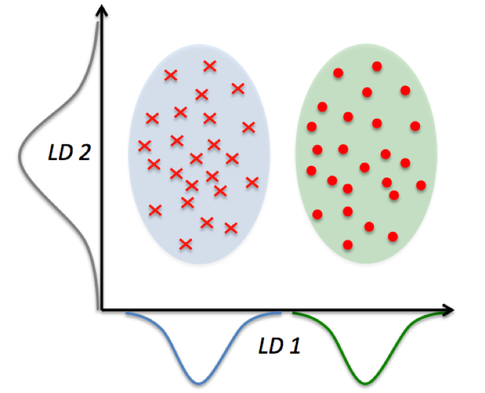
\includegraphics[width=0.4\columnwidth]{lda} }}
	\caption{\\PCA and LDA implemented on 2-dimensional data}
\end{center}
\end{frame}

\begin{frame}
  \frametitle{LDA - classification}
  
  Assumptions:
  \begin{itemize}
  	\item we assume normality for each independent variable
  	\item homogeneity of variance/covariance
  	\item independence between samples
  \end{itemize}

	Classification steps:
	\begin{itemize}
		\item for each class $\mu_i$, we compute 	
		\begin{equation}
		f_i(x_k) = \mu_i {w_a}^{-1} {x_k}^T - \dfrac{1}{2} \mu_i {w_a}^{-1} {\mu_i}^T + ln(P_i)
		\end{equation} 
		\item we classify it to the class with max($f_i(x_k)$)
	\end{itemize}
\end{frame}
%  recursive training algorithm \cite{wiki:c45} :
%  
%  \begin{enumerate}
%  \item check stopping conditions
%    
%    \begin{itemize}
%    \item no more features
%    \item set is smaller than \code{minLeaf}
%    \item all samples in the same class
%    \item no feature improves information gain (IG)
%    \end{itemize}
%  \item iterate over each available feature, perform a line search to approximate the highest IG
%  \item recur over the subsets given by splitting at the feature and threshold with the highest IG 
%  \end{enumerate}
%
%\begin{equation}
%  \mathrm{IG}(X) = \mathrm{H}(X) - \sum_{i=1}^{2} \frac{|S_i|}{|X|} \mathrm{H}(S_i)
%\end{equation}
%
%\begin{equation}
%  \mathrm{H}(X) = -\sum_{i=1}^n {\mathrm{P}(x_i) \log_2 \mathrm{P}(x_i)}
%\end{equation} 
%  
%\end{frame}